% Hybrid decoder interleave (f = 1/8) — TikZ source. Compiles to a tight
% standalone PDF (pdflatex figures/hybrid-interleave.tex), which
% `book-scaffold build-figures` converts to public/figures/hybrid-interleave.svg.
%
% One period of a windowed hybrid stack: 7 recurrent (SSM) blocks each carry a
% FIXED d_s*d state; 1 sliding-window attention layer carries a FIXED 2wd
% window cache. Neither depends on n. Below, the same contrast is redrawn along
% the sequence axis: a constant-width window cache vs. full attention's 2nd
% cache, which grows linearly with n.
\documentclass[tikz,border=3pt]{standalone}
\usepackage{amsmath}
\usepackage{amssymb}
\usepackage{tikz}
\usetikzlibrary{positioning,calc,decorations.pathreplacing,fit}
\begin{document}
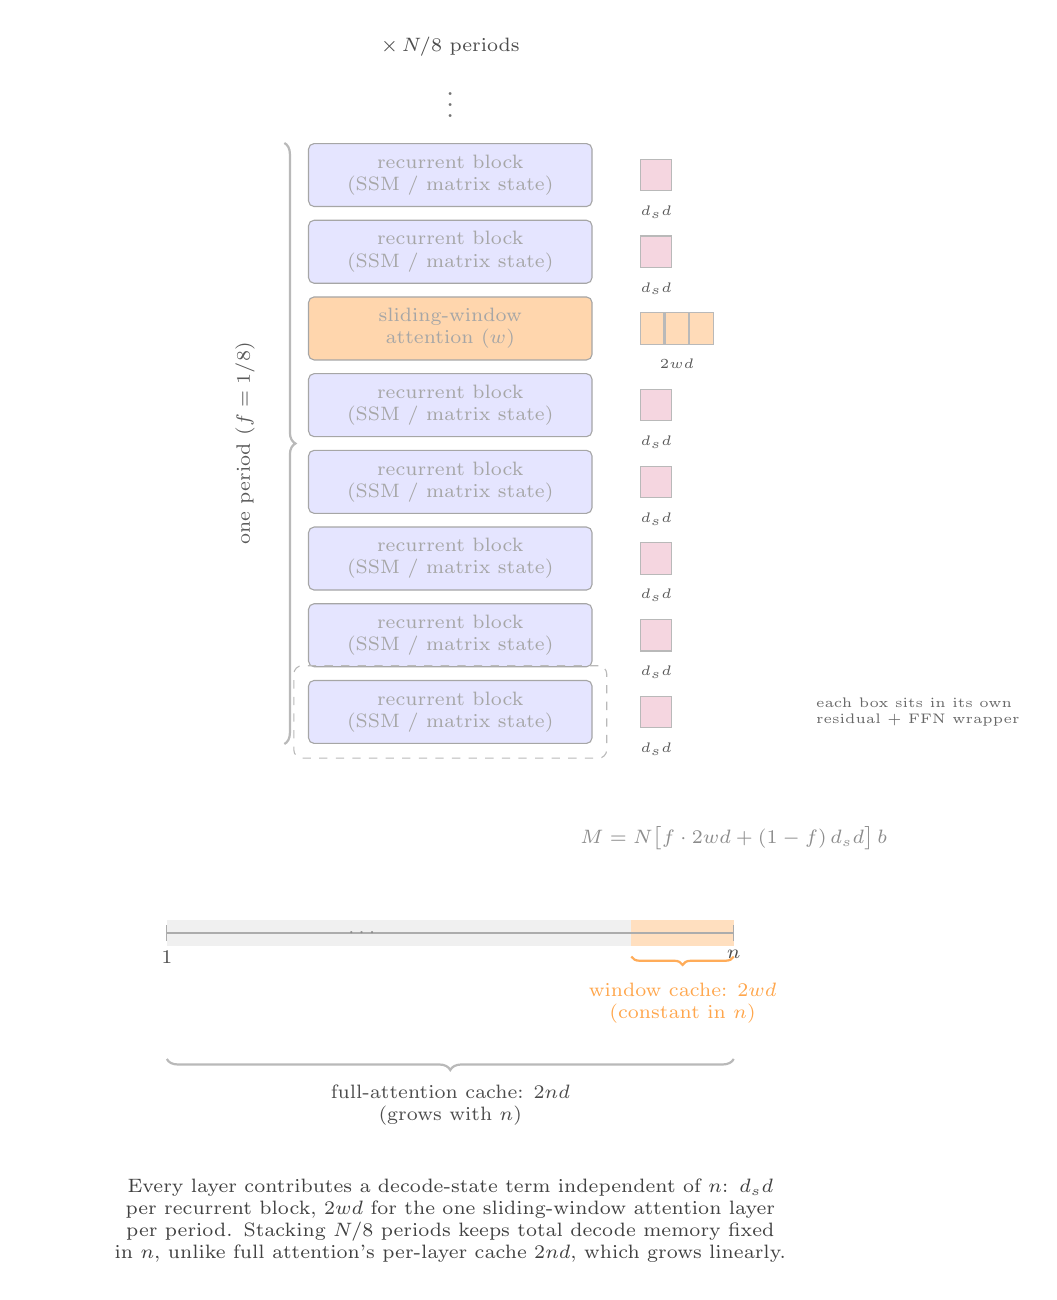
\begin{tikzpicture}[
    font=\small,
    box/.style={draw, gray!70, rounded corners=2pt, align=center,
                minimum width=36mm, minimum height=8mm, inner sep=2pt,
                font=\scriptsize},
    rec/.style={box, fill=blue!10},
    att/.style={box, fill=orange!32},
    sq/.style={draw, gray!55, minimum width=4mm, minimum height=4mm,
               inner sep=0pt, fill=purple!16},
    cell/.style={draw, gray!55, minimum width=3mm, minimum height=4mm,
                 inner sep=0pt, fill=orange!28},
  ]
  % ---------------------------------------------------------------
  % Layer stack, bottom (L1) to top (L8); attention at L6 (3rd from top)
  % ---------------------------------------------------------------
  \node[rec] (L1) {recurrent block\\(SSM / matrix state)};
  \node[rec, above=1.6mm of L1] (L2) {recurrent block\\(SSM / matrix state)};
  \node[rec, above=1.6mm of L2] (L3) {recurrent block\\(SSM / matrix state)};
  \node[rec, above=1.6mm of L3] (L4) {recurrent block\\(SSM / matrix state)};
  \node[rec, above=1.6mm of L4] (L5) {recurrent block\\(SSM / matrix state)};
  \node[att, above=1.6mm of L5] (L6) {sliding-window\\attention ($w$)};
  \node[rec, above=1.6mm of L6] (L7) {recurrent block\\(SSM / matrix state)};
  \node[rec, above=1.6mm of L7] (L8) {recurrent block\\(SSM / matrix state)};

  % state icons + labels (right of each layer): fixed-size square d_s d,
  % except the attention layer, which gets a short band of cells 2wd
  \node[sq, right=6mm of L1] (S1) {};
  \node[below=0.6mm of S1, font=\tiny, text=black!65] {$d_s d$};
  \node[sq, right=6mm of L2] (S2) {};
  \node[below=0.6mm of S2, font=\tiny, text=black!65] {$d_s d$};
  \node[sq, right=6mm of L3] (S3) {};
  \node[below=0.6mm of S3, font=\tiny, text=black!65] {$d_s d$};
  \node[sq, right=6mm of L4] (S4) {};
  \node[below=0.6mm of S4, font=\tiny, text=black!65] {$d_s d$};
  \node[sq, right=6mm of L5] (S5) {};
  \node[below=0.6mm of S5, font=\tiny, text=black!65] {$d_s d$};
  \node[sq, right=6mm of L7] (S7) {};
  \node[below=0.6mm of S7, font=\tiny, text=black!65] {$d_s d$};
  \node[sq, right=6mm of L8] (S8) {};
  \node[below=0.6mm of S8, font=\tiny, text=black!65] {$d_s d$};

  \node[cell, right=6mm of L6] (c1) {};
  \node[cell, right=0mm of c1] (c2) {};
  \node[cell, right=0mm of c2] (c3) {};
  \node[below=0.6mm of c2, font=\tiny, text=black!65] {$2wd$};

  % ---------------------------------------------------------------
  % Top of stack: the period repeats
  % ---------------------------------------------------------------
  \node[above=2mm of L8, font=\normalsize, text=black!55] (dots) {$\vdots$};
  \node[above=0mm of dots, font=\scriptsize, text=black!70]
    {$\times\, N/8$ periods};

  % period brace (left side of the stack)
  \draw[decorate, decoration={brace, amplitude=4pt, mirror}, gray!55, thick]
    ($(L1.south west)+(-3mm,0)$) -- ($(L8.north west)+(-3mm,0)$)
    node[midway, xshift=-5mm, font=\scriptsize, text=black!65, align=center,
         rotate=90] {one period ($f=1/8$)};

  % side legend: every block drawn above is shorthand for a residual + FFN
  % wrapper around it -- mark the bottom block as the representative instance
  \node[draw, gray!55, dashed, rounded corners=3pt, fit=(L1), inner sep=1.8mm]
    (wrap1) {};
  \node[right=17mm of S1, font=\tiny, text=black!60, align=left]
    {each box sits in its own\\residual $+$ FFN wrapper};

  % ---------------------------------------------------------------
  % Sequence axis (below the stack): window cache vs. full-attention cache
  % ---------------------------------------------------------------
  \coordinate (axisMid) at ($(L1.south)+(0,-24mm)$);
  \coordinate (axisL) at ($(axisMid)+(-36mm,0)$);
  \coordinate (axisR) at ($(axisMid)+(36mm,0)$);
  \coordinate (winL) at ($(axisR)+(-13mm,0)$);

  \fill[black!6] ($(axisL)+(0,-1.6mm)$) rectangle ($(axisR)+(0,1.6mm)$);
  \fill[orange!25] ($(winL)+(0,-1.6mm)$) rectangle ($(axisR)+(0,1.6mm)$);
  \draw[gray!65] (axisL) -- (axisR);
  \draw[gray!65] ($(axisL)+(0,-1mm)$) -- ($(axisL)+(0,1mm)$);
  \draw[gray!65] ($(axisR)+(0,-1mm)$) -- ($(axisR)+(0,1mm)$);
  \node[below=1mm of axisL, font=\scriptsize, text=black!70] {$1$};
  \node[below=1mm of axisR, font=\scriptsize, text=black!70] {$n$};
  \node[font=\scriptsize, text=black!45] at ($(axisMid)+(-11mm,0)$) {$\cdots$};

  \draw[decorate, decoration={brace, amplitude=3pt, mirror}, orange!65, thick]
    ($(winL)+(0,-3mm)$) -- ($(axisR)+(0,-3mm)$)
    node[midway, below=2mm, font=\scriptsize, text=orange!70, align=center]
    {window cache: $2wd$\\(constant in $n$)};

  \draw[decorate, decoration={brace, amplitude=4pt, mirror}, gray!55, thick]
    ($(axisL)+(0,-16mm)$) -- ($(axisR)+(0,-16mm)$)
    node[midway, below=2mm, font=\scriptsize, text=black!70, align=center]
    {full-attention cache: $2nd$\\(grows with $n$)};

  % caption formula, tucked unobtrusively in the gap above the axis
  \node[font=\scriptsize, text=black!45] at ($(axisR)+(0,12mm)$)
    {$M = N\big[f\cdot 2wd + (1-f)\,d_s d\big]\,b$};

  % main caption
  \node[below, align=center, text width=10.5cm, font=\scriptsize, text=black!75]
    at ($(axisMid)+(0,-30mm)$)
    {Every layer contributes a decode-state term independent of $n$: $d_s d$ per
     recurrent block, $2wd$ for the one sliding-window attention layer per
     period. Stacking $N/8$ periods keeps total decode memory fixed in $n$,
     unlike full attention's per-layer cache $2nd$, which grows linearly.};
\end{tikzpicture}
\end{document}
